
\cleardoublepage

\noindent{\bf\Huge\color{oblue} Resumen ejecutivo}
\addcontentsline{toc}{chapter}{Resumen ejecutivo}
\vspace{1cm}



\begin{minipage}{0.5\textwidth}

\includegraphics[width = 0.8\textwidth]{recruitement_problem.jpg}
\end{minipage} \hfill
\begin{minipage}{0.45\textwidth}
\noindent{\bf\huge\color{oyellow} El problema}
\medskip

\noindent Encontrar el mejor candidato para una oferta
de trabajo en un entorno cada vez más digitalizado.
¿Es posible usar la información de las redes sociales
para optimizar el proceso?
\end{minipage}
\vspace{1.5cm}


\begin{minipage}{0.7\textwidth}
\noindent {\bf\huge\color{oyellow} Una nueva fuente de información: Twitter}
\medskip

\noindent Usaremos los tuits publicados con contenido relativo 
a la oferta de trabajo, y luego usaremos nuestros algoritmos innovadores para:
\begin{itemize}
\item descubrir en qué lenguajes tuitean los usuarios 
\item descubrir si los tuits seleccionados son relevantes,
y de aquí extraer los usuarios activos en ese perfil
\item descubrir qué usuarios son personas candidatas a la oferta
\end{itemize}
\end{minipage}\hfill
\begin{minipage}{0.4\textwidth}
\begin{tabular}{c}

\includegraphics[width=0.4\textwidth]{twitter-logo-final.png}\\

\includegraphics[width=0.2\textwidth]{flecha.pdf}\\

\includegraphics[width=0.8\textwidth]{rightcandidate.jpg}
\end{tabular}
\end{minipage}
\vspace{1.5cm}


\begin{minipage}{0.4\textwidth}

\includegraphics[width=0.8\textwidth]{candidate_selection.jpg}
\end{minipage}\hfill
\begin{minipage}{0.55\textwidth}
{\bf\huge\color{oyellow} ¿Qué candidatos son los mejores?}
\medskip

\noindent Usaremos dos tipos de algoritmos de ordenación para obtener 
la lista de los mejores candidatos:
\begin{itemize}
\item Por contenido publicado: índice h
\item Por relevancia en la red de usuarios: medidas
de centralidad (por grado, por autovector, Bonacich, PageRank, cercanía e intermediación)
\end{itemize}
\noindent ¡Mira en Shiny la lista ordenada de los usuarios!
\end{minipage}




\begin{sidewaysfigure}
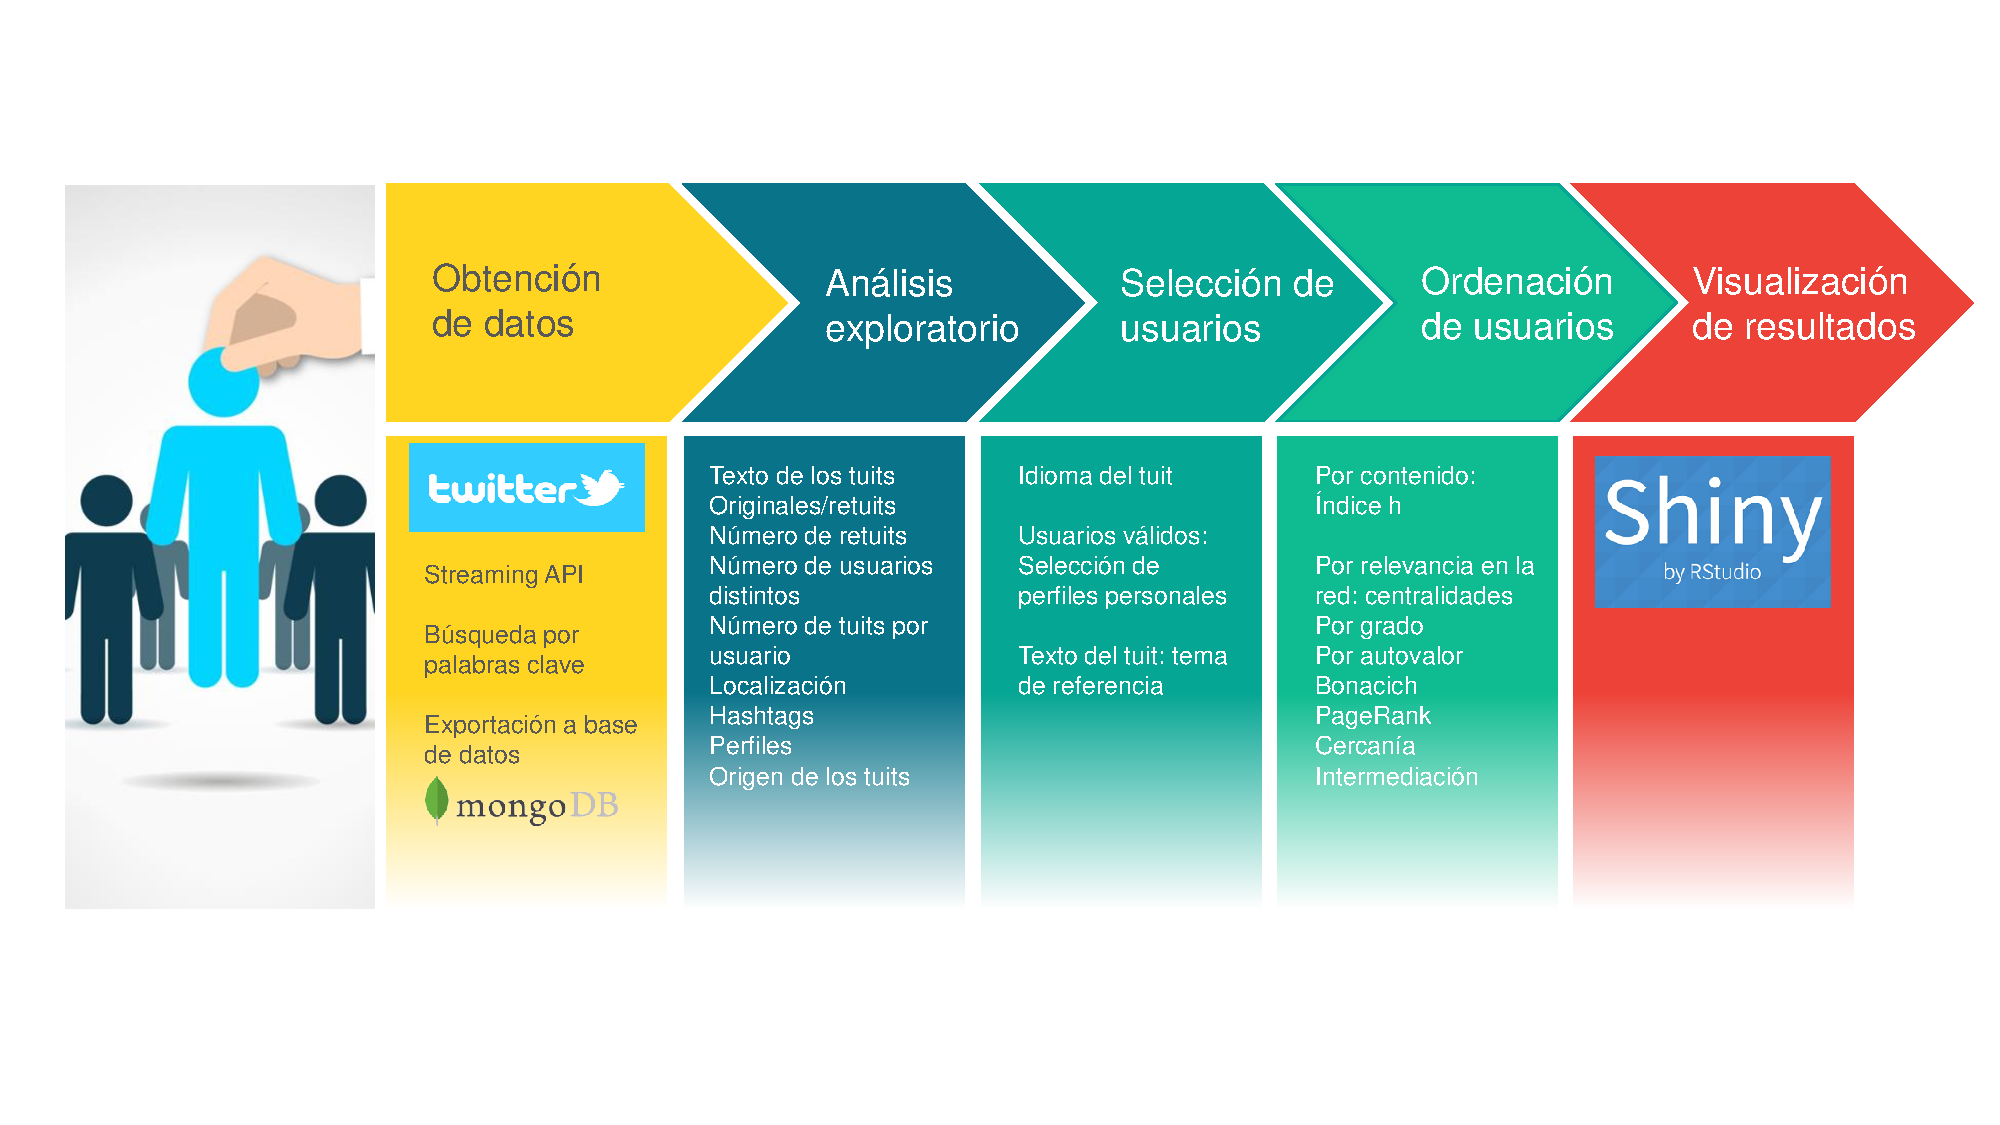
\includegraphics[width=\textwidth]{workflow.pdf}
\caption{Flujo de trabajo esquemático.}
\label{fig:flujo_de_trabajo}
\end{sidewaysfigure}